\chapter{Process and Event}

%%\chapter{Processes}
% \label{chapter-scenario-processes}

\section{Simple Process Sequence}

\textbf{Created by:} Jim Logan \\
\textbf{Modified by:} Jim Logan \\

\subsection*{Scenario Objective}
% Instruction box
This scenario demonstrates how to represent a sequence of time-stamped events using the \textbf{BFO/IOF ontology}. Several use cases are given, where each subsequent use case augments the previous one, culminating in a use case that demonstrates how to determine the type of an overall process automatically from a sequence of sub-processes.

\textit{ 
Note: I'm unsure what to say about the purpose of doing this!
}

\subsection*{General Pattern Description}

This pattern creates instances of \cname{bfo}{process}, each of which
\opname{core}{occupiesTemporalRegion}
one \\
\cname{bfo}{temporalInterval}
with single start and end instances of
\cname{bfo}{TemporalInstant}
that each \\
\opname{core}{hasValueExpressionAtAllTimes} some
\cname{core}{TemporalInstantValueExpression}, according to the earlier pattern in
\ref{sec-clock-calendar}.

\textit{
TBD: Provide a figure containing the pattern independent of the use case (e.g., just measurements in general as opposed to measuring a particular thing such as pH or length).
}
\noindent \textit{This diagram is generally a simple class-relation diagram. Please see examples of class-relation diagram here.}

\textit{ 
Describe the general pattern, including any background why such types and relations are used. Also mention any alternative or shortcuts. Please provide a background of the types and relations in the context of IOF (please prefer logical arguments to didactic arguments).
}


\subsection*{Use Case: Simple Process Sequence}
This first use case is the simplest. It uses the example data, shown below, to create corresponding instances in the IOF theory of what must have existed in the world to justify the data.

 \textit{ 
Describe a concrete use case for the pattern. (Multiple use cases can be described for one pattern. If multiple, please use distinct use case titles and repeat all subsubsections for each use case.)
  }

\newcommand{\ti}{\cname{bfo}{TemporalInstant }}

\subsubsection*{Use-Case Pattern Description}
This use case follows the pattern in \ref{sec-clock-calendar}.
Each timestamp in a row that is marked "Start" creates several instances at once and then wires them together as follows:
a \cname{bfo}{Process} that \opname{core}{occupiesTemporalRegion} a \ti that \opname{bfo}{hasFirstInstant} a \cname{bfo}{TemporalInstant} that \cname{iof}{hasValueExpressionAtAllTimes} a \cname{time}{DateTimeDescription}.

Each timestamp in a row that is marked "Stop" augments what was already created for a "Start" row with several more instances, and then wires them together as follows:
the already-created \cname{bfo}{TemporalRegion} \opname{bfo}{hasLastInstant} a \cname{bfo}{TemporalInstant} that \cname{iof}{hasValueExpressionAtAllTimes} a \cname{time}{DateTimeDescription}.

 \textit{ 
Provide a diagram which matches the use-case pattern description. \\
\noindent \textit{This diagram is generally an object diagram. Please see examples of object diagram here.}
  }

 \textit{ 
Describe how the general pattern is applied to the use case. It is important to highlight within the description how the use-case-specific concepts align with the general pattern (e.g., SubClassOf Class for general pattern).
  }

\subsubsection*{Use-Case Example Data}
The following table shows CSV data resulting from a fictitious machine that makes drip coffee. Each row contains the date and time at which a type of event started or stopped.



\subsubsection*{Data Mapping}
 \textit{ 
Describe how the data was mapped to RDF. Provide an INSERT DATA/ INSERT SPARQL for mapping. Use INSERT only when the use case example data needs further manipulation. \\
For INSERT DATA SPARQL, use only 2/3 records/transactions with named class and individuals. \\
For INSERT SPARQL, declare column names by `\{ \}' to the variable.  
For INSERT query, 
For both, do not use blank nodes.    
  }

\subsubsection*{Data Validation}
 \textit{ 
Data validation can be performed in two ways: accessing interesting facts using SPARQL or validating whether the entire data conforms to the ontology using SHACL. It is preferable to provide both. \\
Provide the SPARQL query in the code block along with the result of the query. \\
  }

\subsection*{Use Case: Typed Process Sequence}
 \textit{ 
Describe a concrete use case for the pattern. (Multiple use cases can be described for one pattern. If multiple, please use distinct use case titles and repeat all subsubsections for each use case.)
  }

\subsubsection*{Use-Case Pattern Description}
 \textit{ 
Provide a diagram which matches the use-case pattern description. \\
\noindent \textit{This diagram is generally an object diagram. Please see examples of object diagram here.}
  }

 \textit{ 
Describe how the general pattern is applied to the use case. It is important to highlight within the description how the use-case-specific concepts align with the general pattern (e.g., SubClassOf Class for general pattern).
  }

\subsubsection*{Use-Case Example Data}
The following table shows CSV data resulting from a fictitious machine that makes drip coffee. Each row contains the date and time at which a type of event started or stopped.

\begin{table}[ht]
    \centering
    \csvautotabular{scenarios/simple-process-sequence/data/EventLog.csv}
    \caption{An Example Event Log for Making Coffee}
    \label{tab:my_label}
\end{table}    


\subsubsection*{Data Mapping}
 \textit{ 
Describe how the data was mapped to RDF. Provide an INSERT DATA/ INSERT SPARQL for mapping. Use INSERT only when the use case example data needs further manipulation. \\
For INSERT DATA SPARQL, use only 2/3 records/transactions with named class and individuals. \\
For INSERT SPARQL, declare column names by `\{ \}' to the variable.  
For INSERT query, 
For both, do not use blank nodes.    
  }

\subsubsection*{Data Validation}
 \textit{ 
Data validation can be performed in two ways: accessing interesting facts using SPARQL or validating whether the entire data conforms to the ontology using SHACL. It is preferable to provide both. \\
Provide the SPARQL query in the code block along with the result of the query. \\
  }

\section*{Material flow in a process design}
This scenario demonstrates how to represent a SysML/UML activity diagram in an IOF Ontology.
Basically, how to show the material flow, i.e., the input and output of the processes.
The use case should include raw materials as input in the first step, intermediate material entities, and the final product, utilizing hasInput and hasOutput along with raw material and product roles.


% \section*{Process Design and Conformance}
%  Here discuss how to classify time stamped events automatically as making coffee.

\section{Algorithm execution}
\label{sec-algorithm-execution}

\section{Algorithm execution}
\label{sec-algorithm-execution}

\textbf{Created by:} Milos Drobnjakovic \\
\textbf{Modified by:} Milos Drobnjakovic \\

\subsection*{Scenario Objective}

This scenario depicts how to express executions of algorithms by using BFO/IOF ontology.

Specifically, this pattern focuses on algorithm executions which produce Information Content Entities (ICEs) as outputs. As such, algorithms that return no ‘outputs’ are not included in this pattern.

This scenario is limited to algorithms that are part of a software system.


\subsection*{General Pattern Description}
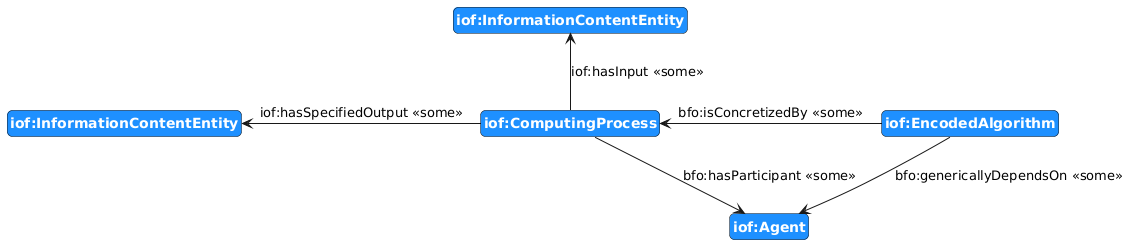
\includegraphics[scale=0.6]{scenarios/algorithm-execution/images/algorithm-execution-general.png}

...

\subsubsection*{Use Case: Drill failure prediction} 
A multilayer perceptron (MLP – a type of a neural network) is used to predict drill failure based on five measured parameters: ‘tool wear’, ‘air temperature’, ‘process temperature’, ‘torque’,’rotational speed’. The model uses the given parameters and outputs either ‘FAIL’ or ‘NOT FAIL’.

\subsubsection*{Use-Case Pattern Description}

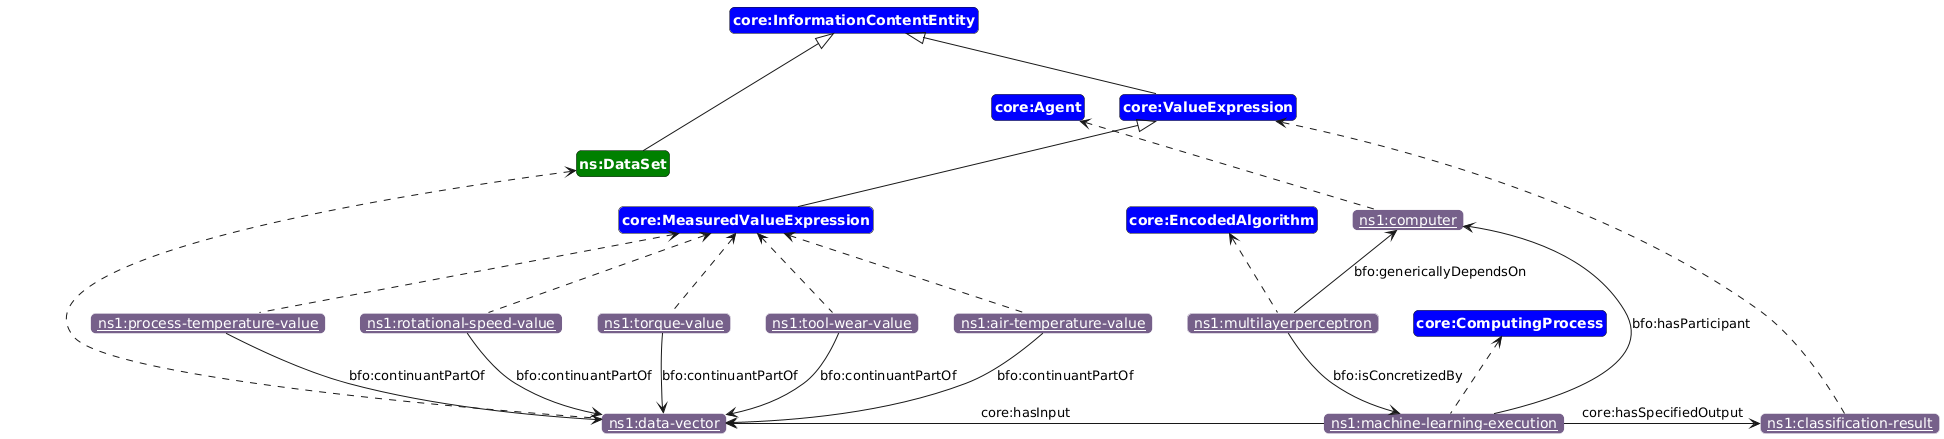
\includegraphics[scale=0.23]{scenarios/algorithm-execution/images/algorithm-execution-usecase1.png}

The machine learning model (MultiLayerPerceptron1) - an instance of:Encoded Algorithm is being concretized in a model execution process - an instance of:Computing Process. The MLP generically depends on a computer system (in this case an instance of Agent) which participates in the model execution process. Model execution utilizes the measured values associated with the drill and the drilling process and produces a ClassificationResult which is an instance of a ValueExpression. Since the objective is to predict machine failure the ClassificationResult is a prediction of the DrillFunction. The ClassificationResult can have two values associated with hasSimpleExpressionValue: 1) FAIL or 2) NOT FAIL. On the diagram bellow an example with the FAIL value is given. For brevity purposes the actual measurement values and their units are excluded from the diagram. Also, the association of the measured values with “drill attributes” or the “drilling process” are omitted. For a detailed guide on connecting the measured values with different entties - the user should see (placeholder link).

\subsubsection*{Use-Case Example Data}

For this use case a publicly available dataset was used: Predictive Maintenance⚙️ 

The dataset is a single CSV table consisting of the columns: ‘tool wear’, ‘air temperature’, ‘process temperature’, ‘torque’,’rotational speed’, ‘process ID, ‘type’ and ‘product ID’, ‘failure type’.

\begin{tabularx}{\textwidth}{|l|X|X|X|X|X|X|X|X|X|X|}
\hline
UDI & Product ID & Type & Air temperature {[}K{]} & Process temperature {[}K{]} & Rotational speed {[}rpm{]} & Torque {[}Nm{]} & Tool wear {[}min{]} & Target & Failure Type \\ \hline
1   & M14860     & M    & 298.1                   & 308.6                       & 1551                       & 42.8            & 0                   & 0      & No Failure   \\
2   & L47181     & L    & 298.2                   & 308.7                       & 1408                       & 46.3            & 3                   & 0      & No Failure   \\
3   & L47182     & L    & 298.1                   & 308.5                       & 1498                       & 49.4            & 5                   & 0      & No Failure   \\ \hline
\end{tabularx}

For prediction purposes, type and Product ID are omitted and are as such not included in the RDF. The exact type of failure is not utilized in this UC, since the model target is binary classification. Finally, `process id' is utilized for IRI construction of the drill.

\subsubsection*{Data Mapping Description}

\begin{verbatim}
INSERT DATA {
    <http://example.org/ns1:freight-train> a <http://example.org/bfo:Entity>;
    <http://example.org/ns1:freight-train> <http://example.org/bfo:locatedInAtSomeTime> 
        <http://example.org/ns1:powder-river-basin>.
}
\end{verbatim}

\subsubsection*{Data Validation}